\documentclass[t,noamsthm]{beamer}

\mode<presentation>
{
  \usetheme{Goettingen}
  \setbeamercovered{transparent}
  \setbeamertemplate{navigation symbols}{}
}

\usepackage[english]{babel}
\usepackage[latin1]{inputenc}
\usepackage[T1]{fontenc}
%\usepackage{arev}

\title[PySMPC]{Python Secure Multi-Party Computation}

\subtitle{High-Level Design Overview}

\author{Martin Geisler}

\institute[BRICS]{
  BRICS\\
  Department of Computer Science\\
  University of Aarhus
}

\date{September 20th, 2007}

% \pgfdeclareimage[height=0.5cm]{university-logo}{university-logo-filename}
% \logo{\pgfuseimage{university-logo}}

% If you wish to uncover everything in a step-wise fashion, uncomment
% the following command: 
%\beamerdefaultoverlayspecification{<+->}

\usepackage{tikz}

\newcommand{\rulecolor}{structure!60}
\newcommand{\fillcolor}{structure!15}

\tikzstyle{player}=[circle,fill=\fillcolor,draw=\rulecolor]


\usepackage{listings}
\lstset{
  language=Python,
  basicstyle=\footnotesize,
  columns=fullflexible,
  showstringspaces=false,
  frame=single,
  rulecolor=\color{\rulecolor},
  backgroundcolor=\color{\fillcolor}
}
\newcommand{\py}[1]{\lstinline|#1|}

\usepackage{nath} \delimgrowth=2

\begin{document}

\begin{frame}
  \titlepage
\end{frame}

%\begin{frame}{Outline}
%  \tableofcontents
%  % You might wish to add the option [pausesections]
%\end{frame}

\section{Features}

\begin{frame}{PySMPC Features}

  \begin{itemize}

  \item API for writing secure multi-party computations
    \begin{itemize}
    \item Simple if you already know Python
    \item A custom language can be added on top of the API
    \end{itemize}

  \item<2-> Efficient asynchronous design
    \begin{itemize}
    \item Automatic parallelism
    \item Single-threaded (no locks!)
    \end{itemize}
    
  \item<3-> Simple architecture
    \begin{itemize}
    \item Small code base (less than 2,000 lines of code)
    \item Few layers of abstraction\dots
    \item \dots but hopefully sufficiently many
    \end{itemize}

  \end{itemize}

\end{frame}

\section{Example}

\begin{frame}{Example MPC Calculation}

  \begin{columns}

    \column{0.5\textwidth}

    \centering
    \begin{tikzpicture}
      \draw (0,0) + (90:2cm) node[player] (P1) {$P_1$}
                  +(210:2cm) node[player] (P2) {$P_2$}
                  +(330:2cm) node[player] (P3) {$P_3$};

      \visible<1>{
        \draw (P1.north) node[above] {$x$};
        \draw (P2.south) node[below] {$y$};
        \draw (P3.south) node[below] {$z$};
      }

      \visible<2>{
        \draw[->] (P1) .. controls +(75:1cm) and +(105:1cm) ..
          node[above,sloped] {$x_1$} (P1);
        \draw[->] (P1) .. controls +(230:1cm) and +(70:1cm) ..
          node[above,sloped] {$x_2$} (P2);
        \draw[->] (P1) .. controls +(-50:1cm) and +(110:1cm) ..
          node[above,sloped] {$x_3$} (P3);

        \draw[->] (P2) .. controls +(50:1cm) and +(250:1cm) ..
          node[below,sloped] {$y_1$} (P1);
        \draw[->] (P2) .. controls +(225:1cm) and +(255:1cm) ..
          node[below] {$y_2$} (P2);
        \draw[->] (P2) .. controls +(10:1cm) and +(170:1cm) ..
          node[above,sloped] {$y_3$} (P3);

        \draw[->] (P3) .. controls +(130:1cm) and +(-70:1cm) ..
          node[below,sloped] {$z_1$} (P1);
        \draw[->] (P3) .. controls +(-170:1cm) and +(-10:1cm) ..
          node[below,sloped] {$z_2$} (P2);
        \draw[->] (P3) .. controls +(-75:1cm) and +(-45:1cm) ..
          node[below] {$z_3$} (P3);
      }

      \visible<3>{
        \draw (P1.north) node[above] {$x_1$, $y_1$, $z_1$};
        \draw (P2.south) node[below,xshift=5pt] {$x_2$, $y_2$, $z_2$};
        \draw (P3.south) node[below,xshift=-5pt] {$x_3$, $y_3$, $z_3$};
      }

      \visible<4>{
        \draw[<->,dashed] (P1) -- (P2);
        \draw[<->,dashed] (P2) -- (P3);
        \draw[<->,dashed] (P3) -- (P1);
      }

      \visible<5-6>{
        \draw (P1.north) node[above] {$r_1$};
        \draw (P2.south) node[below] {$r_2$};
        \draw (P3.south) node[below] {$r_3$};
      }

      \visible<6>{
        \draw[->] (P1) .. controls +(230:1cm) and +(70:1cm) ..
          node[above,sloped] {$r_1$} (P2);
        \draw[->] (P1) .. controls +(-50:1cm) and +(110:1cm) ..
          node[above,sloped] {$r_1$} (P3);

        \draw[->] (P2) .. controls +(50:1cm) and +(250:1cm) ..
          node[below,sloped] {$r_2$} (P1);
        \draw[->] (P2) .. controls +(10:1cm) and +(170:1cm) ..
          node[above,sloped] {$r_2$} (P3);

        \draw[->] (P3) .. controls +(130:1cm) and +(-70:1cm) ..
          node[below,sloped] {$r_3$} (P1);
        \draw[->] (P3) .. controls +(-170:1cm) and +(-10:1cm) ..
          node[below,sloped] {$r_3$} (P2);
      }

      \visible<7>{
        \draw (P1.north) node[above] {$r$};
        \draw (P2.south) node[below] {$r$};
        \draw (P3.south) node[below] {$r$};
      }

    \end{tikzpicture}

    \column{0.5\textwidth}

    \begin{itemize}
    \item<1-> Players $P_1$, $P_2$, and $P_3$
    \item<2-> Sharing $x$, $y$, and $z$
    \item<4-> Computes $r= (x+y)\cdot z$
    \item<6-> Opens the result $r$
    \end{itemize}

  \end{columns}
\end{frame}

\begin{frame}{Example PySMPC Program}

\begin{columns}
  \column{0.57\textwidth}

  \lstinputlisting[linerange={1-5}]{example.py}
  \vspace{-0.5\baselineskip}
  \uncover<2->{\lstinputlisting[linerange={7-9}]{example.py}}
  \vspace{-0.5\baselineskip}
  \uncover<3->{\lstinputlisting[linerange={11-13}]{example.py}}
  \vspace{-0.5\baselineskip}
  \uncover<4->{\lstinputlisting[linerange={15-17}]{example.py}}

  \column{0.43\textwidth}

  \begin{itemize}[<+->]
  \item Import statements
  \item Load configuration
  \item Create Runtime, share and calculate
  \item Open and print result
  \end{itemize}
\end{columns}

\end{frame}

\begin{frame}{Example Configuration File}

  \lstdefinelanguage{ini}{
    morecomment=[l]{\#},
    moredelim=[s][\textbf]{[}{]},
    moredelim=[s][\textbf]{[[}{]]},
    moredelim=[s][\textbf]{[[[}{]]]}
  }

  \lstinputlisting[language=ini]{sample-config.ini}

\end{frame}

\section{Scheduling}

\begin{frame}{Asynchronous Design}

  \begin{columns}

    \column{0.3\textwidth}

    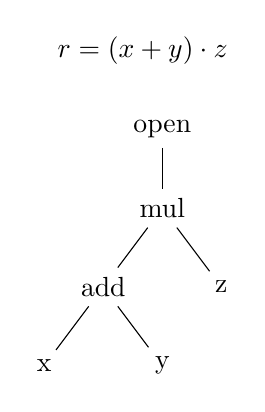
\begin{tikzpicture}
      \tikzstyle{level 1}=[level distance=10mm]

      \draw (-0.25,0) node {$r = (x+y) \cdot z$};
      \draw (0,-0.5) node[xshift=-0.75pt,rotate=-90] {$\rightsquigarrow$};

      \draw (0,-1) node {open}
        child {node {mul}
          child {node {add}
            child {node {x}}
            child {node {y}}
          }
          child {node {z}}};
    \end{tikzpicture}

    \column{0.7\textwidth}

    \begin{itemize}
    \item Entire tree is scheduled as once
    \item Operations wait on their operands
    \item Results are sent when ready
    \item Result is a form of ``greedy scheduling''
    \item Implicit synchronization, no rounds
    \end{itemize}

  \end{columns}

\end{frame}

\begin{frame}{Greedy Scheduling}
  Advantages:
  \begin{itemize}
  \item At least as efficient as round-based scheduling
  \item No cost when adding new primitives (modular design)
  \item Automatic parallelism
  \end{itemize}

  Disadvantages:
  \begin{itemize}
  \item Not yet proven secure\dots
  \item Somewhat complicated to keep track of operations
  \end{itemize}
\end{frame}


\section{Current Status}

\begin{frame}{What is Implemented?}
  \begin{itemize}
  \item Shamir sharing
  \item PRSS
  \item Opening
  \item Addition, multiplication, exclusive-or
  \item Classic SCET comparison
  \end{itemize}
\end{frame}


\begin{frame}{Assumptions}
  
  Current primitives assume:
  \begin{itemize}
  \item Fixed number of players
  \item Passive and static adversary
  \item Threshold adversary structure, $t < \frac n 2$
  \end{itemize}

  
\end{frame}

\section{Conclusion}

\begin{frame}{Conclusion}

\begin{itemize}
\item PySMPC offers a light-weight design for doing MPC
\item Asynchronous design gives automatic parallelism
\end{itemize}

Installation instructions:
\begin{itemize}
\item $\sim$mg/simap/pysmpc/INSTALL
\end{itemize}

\visible<2>{
  \begin{center}
    \bigskip
    \begin{tikzpicture}
      \draw node[rectangle,draw=\rulecolor,fill=\fillcolor,
        inner sep=2.5em,font=\huge\bfseries] {Questions?};
    \end{tikzpicture}
  \end{center}
}

\end{frame}



\end{document}

% LocalWords:  PySMPC API MPC PRSS SCET
